%%%%%%%%%%%%%%%%%%%%%%%%%%%%%%%%%%%%%%%%%%%%%%%%%%%%%%%%%%%
% --------------------------------------------------------
% Rho
% LaTeX Template
% Version 2.1.1 (01/09/2024)
%
% Authors: 
% Guillermo Jimenez (memo.notess1@gmail.com)
% Eduardo Gracidas (eduardo.gracidas29@gmail.com)
% 
% License:
% Creative Commons CC BY 4.0
% --------------------------------------------------------
%%%%%%%%%%%%%%%%%%%%%%%%%%%%%%%%%%%%%%%%%%%%%%%%%%%%%%%%%%%

\documentclass[9pt,a4paper,twoside,english]{class/backend}
\usepackage[english]{babel}

\setbool{rho-abstract}{true} 
\setbool{corres-info}{true}

%----------------------------------------------------------
% TITLE
%----------------------------------------------------------

\journalname{Numerics}
\title{Générateur de nombres pseudo-aléatoires ou comment produire de l'aléatoire avec un système déterministe ?}

%----------------------------------------------------------
% AUTHORS AND AFFILIATIONS
%----------------------------------------------------------

\author[1]{Duzés Florian}


%----------------------------------------------------------

\affil[1]{Étudiant de master Cryptologie et Sécurité Informatique}


%----------------------------------------------------------
% DATES
%----------------------------------------------------------

\dates{Document rédigé le \today.}

%----------------------------------------------------------
% FOOTER INFORMATION
%----------------------------------------------------------

\leadauthor{Duzés Florian}
\footinfo{Creative Commons CC BY 4.0}
\smalltitle{Numerics}
\institution{Université de Bordeaux}
\theday{\today}

%----------------------------------------------------------
% ARTICLE INFORMATION
%----------------------------------------------------------

\license{Ce document est sous la licence Creative Commons CC BY 4.0.}

%----------------------------------------------------------
% ABSTRACT
%----------------------------------------------------------

\begin{abstract}
    Étude sur les générateurs de nombres pseudo-aléatoires dans le cadre de l'Unité d'enseignement optionnelle Numerics. Ce document retrace brièvement  l'histoire de la création de ces outils, leur multiplicité et leur usage.

\end{abstract}

%----------------------------------------------------------

\begin{document}
	
    \maketitle
    \thispagestyle{firststyle}
    % \tableofcontents
    \linenumbers

%----------------------------------------------------------

\section{Introduction}

    \rhostart{J}'aime jouer aux jeux de société. Et je ne suis pas le seul, car il semble que neuf Français sur dix \cite{jeuxSociete} s'adonnent à cette activité régulièrement. C'est une activité stimulante, qui permet de développer nos liens sociaux et nous offre des occasions de nous challenger intellectuellement. Ainsi, la défaite permet d'établir un bref classement des capacités de chacun. Pourtant, au regard de celle-ci, a-t-on vraiment perdu face à un adversaire plus fort ou face à un hasard capricieux ? Cette remarque prend une ampleur différente si des sommes d'argent sont engagées dans la partie... 

    Aujourd'hui, il est possible de jouer aux cartes sur un ordinateur. Or, un ordinateur est un système déterministe, obéissant à une suite finie d'instructions. Comment, dans ce contexte, peut-on garantir que la distribution des cartes ou d'autres éléments aléatoires reste équitable et imprévisible ?

    Cette question nous amène à explorer le concept des générateurs de nombres pseudo-aléatoires. Ces outils sont essentiels pour simuler ou générer de l'aléa. Ils sont utilisés dans divers domaines, allant de la cryptographie aux simulations scientifiques, en passant par les jeux vidéo et les applications statistiques.

\section{Nature d'un générateur de nombre pseudo-aléatoire}

    \subsection{Définition}
        \begin{rhoenv}[frametitle={Donald E.Knuth, \citetitle{RefGen}}]
        Les séquences générées de manière déterministe sont généralement appelées séquences pseudo-aléatoires ou quasi-aléatoires [\dots], étant entendu qu'elles ne sont aléatoires qu'en apparence. De toute façon, le fait d'être « apparemment aléatoire » est peut-être tout ce que l'on peut dire d'une séquence aléatoire.
        \end{rhoenv}

    Un générateur de nombres pseudo-aléatoires (\textit{PRNG}) est un algorithme qui génère une séquence de nombres présentant certaines propriétés du hasard. \cite{Wiki}
    
    Un PRNG génère des suites de nombres qui ne peuvent pas satisfaire complètement les critères mathématiques qualifiant les suites aléatoires. On les appelle suites pseudo-aléatoires, car leurs propriétés s'approchent seulement des propriétés idéales des suites aléatoires parfaites.
    
    Si l'on souhaite obtenir des nombres aléatoires, il faut qu'ils soient générés d'une source chaotique. La qualité de la source dépend de la qualité du chaos produit par la source. Écouter le bruit électronique d'une résistance ou observer un mur de lampes à lave \cite{lavarand} sont des solutions actuellement utilisées.

    
    \subsection{Caractéristiques}

    \begin{rhoenv}[frametitle={Clifford A. Pickover, \citetitle{CPCB}}]
    La génération de nombres aléatoires est trop importante pour être laissée au hasard.
    \end{rhoenv}
    
    Voici les caractéristiques d'un PRNG :
    \nolinenumbers
    \vspace{-1em}
    \begin{multicols}{2}
        \begin{enumerate}
            \item Déterminisme
            \item Périodicité
            \item Longueur de la période
            \item Uniformité
            \item Indépendance
            \item Qualité statistique
            \item Efficacité calculatoire
            \item Sécurité
            \item Portabilité
        \end{enumerate}
    \end{multicols}
    \linenumbers
    Ces caractéristiques découlent du caractère déterministe de nos algorithmes. Les autres points découlent du domaine de l’analyse de suites numériques.
    Du domaine des suites numériques car, avec un PRNG et une entrée (graine), si l'on utilise la sortie comme nouvelle entrée, on obtiendra une suite numérique que l'on pourra analyser. 

    Et comme c'est déterministe, pour une même graine, la séquence générée sera toujours identique.

    \smallskip

    La périodicité et la longueur de cette période permettent de qualifier la qualité d'un PRNG. Dans le cadre de la cryptologie, on souhaite utiliser de longues périodes pour réduire la prévisibilité du terme suivant.
    
    L'uniformité et l'indépendance des nombres générés permettent de distinguer un bon d'un mauvais PRNG. Les nombres doivent être uniformément distribués sur l'intervalle de sortie et statistiquement indépendants les uns des autres. Ces caractéristiques garantissent que, lors d'une application dans le cadre de simulations ou de tests statistiques, les nombres obtenus sont représentatifs et non biaisés.
    
    Enfin, l'efficacité calculatoire d'un PRNG, sa sécurité et sa portabilité servent à déterminer son usage. Dans le cas des GPS, on souhaite un PRNG qui produise une suite de nombres très rapidement pour permettre de synchroniser deux appareils et calculer leur distance dans l'espace \cite{Wiki}.


\section{Un bref historique}

    \subsection{Origines et premières itérations}\smallskip

    \hspace{10pt}À l'origine, lorsque des scientifiques avaient besoin de nombres aléatoires, ils tiraient des nombres d'une urne équilibrée, tiraient des cartes ou lançaient manuellement des dés \cite{RefGen}. En 1927, une table de (41 600) nombres aléatoires est publiée pour la toute première fois \cite{historique}. C'est le premier travail de simplification et d'accessibilité qui est offert au monde scientifique. Par la suite, une multitude de tables vont fleurir pour améliorer les travaux et les études utilisant l'aléatoire. En 1955, une association américaine, RAND, publie la première table d'un million de nombres \cite{RAND}.
    
    \begin{figure}
        \centering
        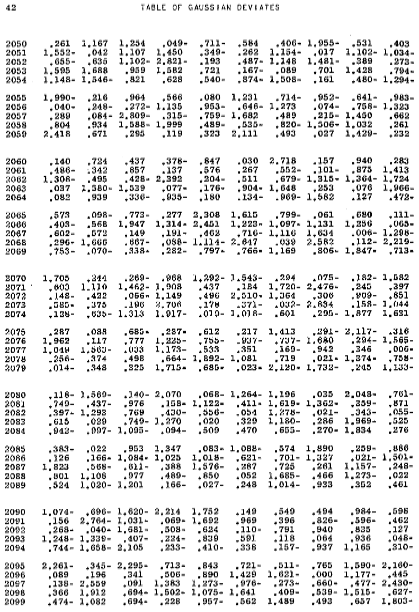
\includegraphics[width=0.5\linewidth]{figures/page_du_RAND_1000000digits.png}
        \caption{Page prise au hasard du \textit{A Million Random Digits with 100,000 Normal Deviates},RAND}
        \label{fig:RAND_page}
    \end{figure}
    
    En parallèle, la technique pour la génération de nombres aléatoires progresse aussi et ERNIE (\textit{Electronic Random Number Indicator Equipment}) fut achevé en 1957. Cette machine servait à tirer les numéros du loto anglais. La génération de nombres est réalisée avec l'observation du bruit produit par le passage d'un courant électrique dans des tubes à néons. ERNIE 1 était capable de générer environ 2 000 nombres par heure. En 2019, ERNIE 5 est entré en activité et observe le bruit quantique, actuellement une des méthodes les plus sûres et les plus imprévisibles pour générer des nombres aléatoires. ERNIE 5 peut générer environ 1,2 million de nombres par heure. \cite{ERNIE}
        
    
    \subsection{Évolutions}\smallskip

    \hspace{10pt}L'utilisation de tables de chiffres était compliquée due au support de l'information, alors sur bande magnétique. Entrer les données est fastidieux et obtenir une table de nombres aléatoires assez grande pour réaliser plusieurs expériences différentes et indépendantes est difficile. L'utilisation d'une machine comme ERNIE n'est pas une solution valide, comment reproduire les résultats obtenus lorsqu'une machine génère des nombres aléatoirement ?
    
    Ce sont ces problématiques, en plus de la démocratisation des ordinateurs dans les milieux scientifiques, qui ont fait avancer les travaux sur les PRNG. Le premier PRNG fut élaboré par Von Neumann en 1946 et se nomme le \textbf{carré médian} \cite{VN_algo}. 
    
    \begin{rhoenv}[frametitle = {\citetitle{VN_algo}}]
        Pour la graine "1111":
        \begin{enumerate}
            \item $1111^2 = 1234321 \implies 12 \ '3432'\ 1 $
            \item $3432^2 = 11778624 \implies 11\ '7786'\ 24 $
        \end{enumerate}
        0n obtient "7786" en deux tours.
    \end{rhoenv}
    
    
    Ce premier PRNG s'est démocratisé assez rapidement et fut largement étudié durant les années 50. Aujourd'hui, il n'est plus utilisé, car il s'avère que c'est une méthode qui dégénère en séquence cyclique, souvent avec une période très courte \cite{SyposiumMonteCarlo}.


\section{Éventails de générateurs de nombres pseudo-aléatoires}

    \hspace{10pt}Tous les types différents de générateurs pseudo-aléatoires mentionnés par la suite sont issus de cet ouvrage : \citetitle{MonteCarloPRNG} \cite{MonteCarloPRNG}.\smallskip
    
    \subsection{Générateurs Congruentiels}\smallskip

    \hspace{10pt}Après la méthode du carré médian, les recherches se sont portées vers l'usage des récurrences linéaires, mais la qualité du PRNG dépend excessivement de la caractérisation de ses paramètres $a_j, b, P$.
     
        \begin{equation}{\text{Récurrence linéaire : }}
            x_{i+1} \equiv a_0 x_i + \cdots + a_j x_{i-j} + b \ (\text{mod} \ P)    
        \end{equation}
    
    Lorsqu'on analyse un PRNG issu de cette méthode, on constate que les  périodes sont trop courtes et présentent des propriétés statistiques insuffisantes. Pourtant, en reprenant cette idée et en la plaçant dans l'espace des multiplications; selon M.Lehmer \cite{lehmer}, alors on obtient un \textbf{générateur congruentiel multiplicatif (MCG)} :
        \begin{equation}
            x_{i+1} \equiv \lambda \cdot x_i \ (\text{mod} \ P)
        \end{equation}

    La forme $(1)$ récurrence linéaire est trop générale et n'est pas satisfaisante pour des travaux statistiques. En revanche, en la déclinant en $(2)$ on obtient plus facilement de meilleures propriétés.
    
     En 1988, Park et Miller \cite{ParkMiller} ont proposé un PRNG en définissant $P$ comme un premier de Mersenne et $\lambda$ une racine modulo 31 :
        \begin{equation}
            x_{i+1} \equiv 7^5 \cdot x_i \ (\text{mod} \ 2^{31} - 1)
        \end{equation}
    
    Ce PRNG se nomme \textbf{MINSTD} et a été utilisé dans Carbon (vieille API d'Apple) et C++11 (C++ version 2011).
    
    
    En poursuivant cette voie, les \textbf{Générateurs récursifs multiples (MRG)} ont été développés pour obtenir une période plus importante que les MCG. Messieurs Marsaglia et Zaman \cite{Multiply&Carry} ont conçu une variation des MRG nommée \textit{Multiply with carry}. Malheureusement, il a été démontré quelques années plus tard que cette variante produit des séquences identiques à des MCG.
    
    \subsection{Générateurs à rétroaction}\smallskip

    \hspace{10pt}Les équations linéaires, c'est chouette, mais dans un contexte informatique, où tout se réduit à des bits, où les nombres sont transformés et évalués en base 2, n'y a-t-il moyen d'exploiter cette idée pour fabriquer des nombres ?
    Ainsi, Tausworthe a présenté un PRNG \cite{Tausworthe} qui se base sur la manipulation des registres où sont stockés les bits. Cette méthode est en réalité identique à l'équation (1) avec $P = 2$ :
    
        \begin{equation}
            b_i = a_1 b_{i-1} + \cdots + a_j b_{i-j} \ (\text{mod} \ 2)
        \end{equation}
    
    Cette méthode est très rapide mais présente des soucis de sécurité. Par exemple, pour l'équation (4), on sait que sa période maximale est $2^j-1$ (on a j bits et deux choix à chaque fois). En revanche, si l'implémentation est correctement réalisée, alors ces PRNG sont totalement utilisables.
    
    Les itérations suivantes ont ajouté l'idée de décalage entre les bits impactés, puis enfin l'idée de "tordre" les suites de bits. En ajoutant une matrice binaire ($A$) dans les opérations, on peut modifier les résultats et ainsi obtenir une période maximale plus élevée :
    
        \begin{equation}
            y_{i+n} = y_{i+m} \oplus A y_i \text{ ; } n > m 
        \end{equation}
    
    On peut retrouver une implémentation exploitant cette idée dans la bibliothèque \textit{random} de Python. Elle a été conçue en 1998 par Matsumoto et Nishimura \cite{MersenneTwister}, utilise un premier de Mersenne et a une période de $2^{19937}-1$ : le "\textbf{Mersenne Twister}".
    
    \subsection{Générateurs non linéaires}\smallskip

    \hspace{10pt}Le point négatif des PRNG basés sur la récursion linéaire est qu'ils présentent des structures de réseaux. Cette structure peut être problématique si l'on souhaite générer des clés de chiffrement pour une communication, par exemple.
    
    Pour résoudre cette problématique, Lenore Blum, Manuel Blum et Michael Shub ont proposé leur solution \cite{BlumBlumShub} :
    
        \begin{equation}{\textbf{Blum Blum Shub }:}
            \ x_{i+1} = {x_i}^2\ (\text{mod} \ M)
        \end{equation}
    
    Avec M est le produit de deux grands nombres premiers. Le point négatif de ce PRNG est sa lenteur. En revanche, son absence de structure lui a permis d'être utilisée dans des applications cryptographiques. 
    
    \subsection{Générateurs combinaison}\smallskip

    \hspace{10pt}Enfin, la dernière méthode pour concevoir un PRNG et qui permet d'améliorer les propriétés et la période d'un PRNG est de combiner deux ou plusieurs PRNG indépendants.
        
        \begin{equation}
            \theta_i = \frac{x_i}{30 269} + \frac{y_i}{30 307} + \frac{z_i}{30 323} \ (\text{mod} \ 1)
        \end{equation}
    
    Dans cet exemple, trois générateurs congruentiels multiplicatifs sont combinés, il s'agit du PRNG de Wichmann et Hill \cite{WichmannHill}.
    


\section{Tests et étude de qualité}\smallskip

    \hspace{10pt}J'ai mentionné précédemment qu'il était possible d'évaluer les qualités statistiques d'un PRNG. Or ce que l'on a à observer ce sont des suites de nombres. Et rien d'autre qu'une suite de nombres apparemment aléatoire ne ressemble plus à une suite aléatoire, regardez $\pi$.

    \begin{rhoenv}[frametitle = {\textit{Scientific American}, \citetitle{refPI}, Martin Gardner, 1965}]
        Les mathématiciens considèrent le développement décimal de $\pi$ comme une série aléatoire, mais pour un numérologue moderne, il est riche en motifs remarquables.
    \end{rhoenv}

    Pour résoudre ce problème, des algorithmes ont été mis au point pour évaluer la distribution, la présence de corrélation et d'autres éléments à évaluer.

    \subsection{Test Statistiques}\smallskip

    \hspace{10pt}Ces tests permettent de vérifier si les nombres générés sont uniformément distribués et s'ils présentent des corrélations indésirables. La réponse de ces tests n'est pas si une suite est ou n'est pas aléatoire. La réponse est sa probabilité d'être une distribution uniforme.

    \subsubsection{Tests Théorique}\smallskip

    \hspace{10pt}Le \textbf{test spectral} conçus par Coveyou et MacPherson \cite{spectralTest}. Ce test détermine si une suite de $s$ éléments issus d'un PRNG de classe MCG est issue de variables aléatoires indépendantes et uniformément distribuées. Le test utilise une transformée de Fourier sur chaque suite pour l'évaluer. Si la période est $m$ alors chaque $s$-uples doit apparaître $\frac{1}{m^s}$.

   Ce test a été amélioré en 2002 par travailler empiriquement \cite{EmpiricalSpectraltest}. Cette version examine la structure de réseau de la génération du PRNG, il observe la discrépance\footnote{Discrépance : (Mathématiques) Décrit la déviation, parfois asymptotique, d'une situation considérée comme régulière.} maximale par rapport au nombre attendu d'occurrences d'un $s$-uples.
    

    \subsubsection{Tests Empiriques}

    Les tests empiriques consistent à observer le comportement d'un PRNG sur son comportement à grande échelle, avec une mise en perspective de toutes ces productions. Trois tests sont mentionnés ici \cite{MonteCarloPRNG} : \textit{Test d’équidistribution}, \textit{Test sériel} et \textit{Test des séries ascendantes et descendantes}. 
    
    Le test d'équidistribution, où l'intervalle (0, 1) est divisé en k sous-intervalles. Le nombre de valeurs tombant dans chaque sous-intervalle est déterminé pour une séquence de nombres pseudo-aléatoires, et un test khi carré est effectué pour vérifier si les nombres sont uniformément distribués dans leurs intervalles.

    \begin{rhoenv}[frametitle = {Test du khi carré ou $\chi^2$ \cite{khi-deux}}]
        \[
            \chi^2 = \sum_{i, j} \frac{(O_{ij} - E_{ij})^2}{E_{ij}}
        \]
        \begin{itemize}
            \item \( \chi^2 \) : valeur du khi carré,
            \item \( O_{ij} \) : valeur observée,
            \item \( E_{ij} \) : valeur attendue.
        \end{itemize}
        Le test du khi-carré d'adéquation vérifie si nos échantillons correspondent à une distribution définie a priori.
    \end{rhoenv}

    Le test sériel est un autre test empirique important. Il vérifie l'interdépendance entre les nombres pseudo-aléatoires successifs dans une séquence. L'espace est divisé en $r^s$ partitions, et la fréquence avec laquelle les $s$-tuples tombent dans chaque partition est mesurée. Les nombres vraiment aléatoires sont uniformément distribués dans l'espace de dimension $s$, donc une valeur de $\chi^2$ peut être calculée pour évaluer la qualité du générateur.

    Le test des séries ascendantes et descendantes compare la magnitude d'un nombre pseudo-aléatoire avec le précédent. Il compte le nombre de séries ascendantes (ou descendantes) de différentes longueurs dans une séquence de nombres pseudo-aléatoires. Ce test permet de détecter des corrélations indésirables dans les séquences générées. 

     \begin{figure}[h]
        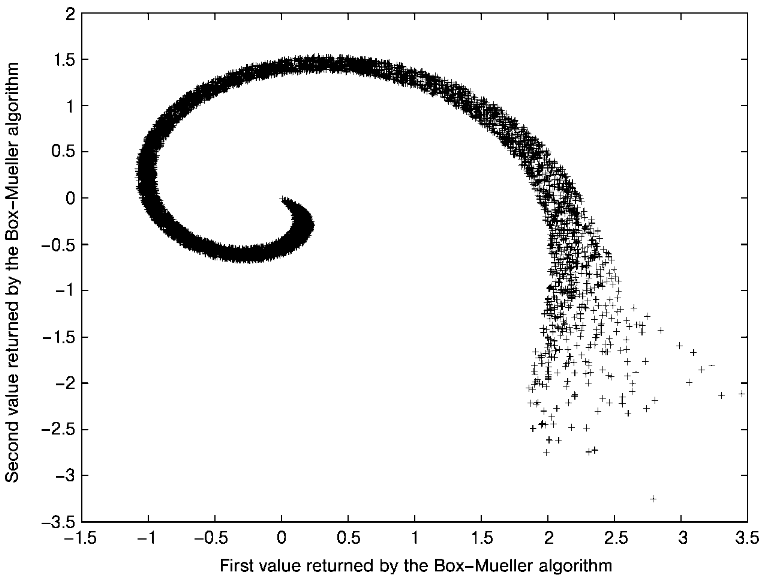
\includegraphics[width=0.5\linewidth]{figures/test_BadPRNG.png}
        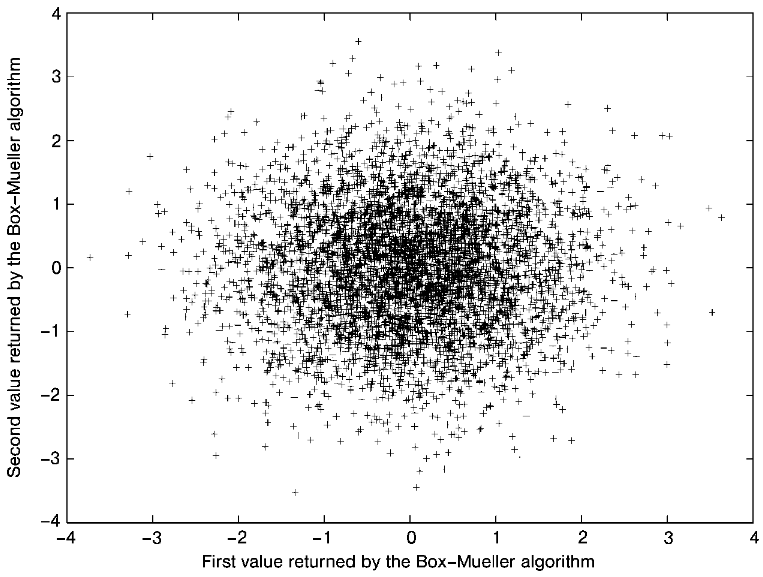
\includegraphics[width=0.5\linewidth]{figures/test_GoodPRNG.png}
        \caption{Extrait de \citetitle{MonteCarloPRNG} présentant deux distributions issus de PRNG dans un objectif de comparaisons de leur qualité}
        \label{fig:PRNG}
    \end{figure}
    
    \subsection{Test de sécurité}

    \hspace{10pt}Les tests de sécurité des PRNG interviennent pour garantir que les nombres générés soient peu prédictibles et donc, ne présentent pas de vulnérabilités exploitables. En utilisant une combinaison de tests théoriques et empiriques, l'objectif est de vérifier si notre PRNG présente une distribution pseudo-uniforme avec aucune période courte, ni de corrélations entre les nombres générés. L'objectif est de se prémunir de la cryptanalyse que peuvent subir nos PRNG et ainsi offrir une faille lors de la génération de clés secrètes utilisées dans les applications sécurisées.


\section{Applications des PRNG}

    \hspace{10pt}Les PRNG sont associés au développement des ordinateurs. Leurs usages s'inscrivent dans le besoin de reproduction de l'aléatoire dans un contexte déterministe. Les trois domaines principaux qui me viennent sont :
    \begin{itemize}
        \item \textit{La cryptographie} - besoin de l'aléatoire pour y dissimuler de l'information.
        \item \textit{Le divertissement} - pour concevoir des jeux avec des comportements imprédictibles.
        \item \textit{La simulation, modélisation} - dans différents domaines scientifiques comme la physique, la finance ou les statistiques.
    \end{itemize}

\section{Un regard sur l'horizon}

    \hspace{10pt}Voici maintenant un siècle que ce domaine s'affine, se perfectionne et progresse. On a un cadre qui nous permet de définir les usages pour lesquels un nouveau PRNG serait applicable. Si je suis imprédictible, je serai utilisé en cryptographie, en revanche si je suis calculable rapidement, j'irai vers des usages statistiques. 

    SHISHUA \cite{shishua} conçu en 2020, est capable de produire un gigabit de nombres par seconde. La construction de ce PRNG est optimisée pour des ordinateurs d'architecture \textit{x86-64}. Dernièrement (ce 31 décembre 2024), une équipe internationale a mis au point un PRNG matériel \cite{wu2024pseudorandomnumbergeneratormultisequence} conçu pour générer simultanément plusieurs séquences non corrélées, avec des statistiques programmables adaptées aux besoins spécifiques des applications. Ce PRNG occupe une surface d'environ 0,0013 mm$^2$ et consomme une énergie de 0,57 pJ/bit.


    Actuellement, l'objectif principal est d'améliorer surtout les structures de PRNG imprédictibles. Les propriétés d'imprédictibilité sont encore mal définies. Ces travaux sont importants pour pouvoir améliorer les performances d'applications cryptographiques.
    
    
    


\section{Conclusion}

\hspace{10pt}À travers ce document, nous avons exploré l'évolution historique et technique des PRNG, leurs nombreuses variantes, ainsi que les tests qui permettent d'évaluer leur performance. La génération de nombres pseudo-aléatoires est un domaine qui allie science, technique et inspiration. Si les PRNG ont largement évolué depuis leurs premières itérations, leur utilisation dépend toujours de compromis entre efficacité, sécurité et qualité statistique. Comprendre leurs caractéristiques et leurs limitations est essentiel pour garantir leur bon usage, que ce soit dans les jeux, la simulation ou la cryptographie. À travers cette exploration, nous avons vu que bien que la perfection de l'aléatoire reste hors de portée, les progrès réalisés nous permettent de répondre à des besoins toujours plus complexes et exigeants.


%----------------------------------------------------------

\printbibliography

%----------------------------------------------------------

\end{document}